%%%%%%%%%%%%%%%%%%%%%%%%%%%%%%%%%%%%%%%%%
% Masters/Doctoral Thesis 
% LaTeX Template for IIIT Allahabad Students
%%%%%%%%%%%%%%%%%%%%%%%%%%%%%%%%%%%%%%%%%

%----------------------------------------------------------------------------------------
%	PACKAGES AND OTHER DOCUMENT CONFIGURATIONS
%----------------------------------------------------------------------------------------

\documentclass[
12pt, % The default document font size, options: 10pt, 11pt, 12pt
oneside, % Two side (alternating margins) for binding by default, uncomment to switch to one side
english, % ngerman for German
singlespacing, % options: singlespacing, onehalfspacing or doublespacing
liststotoc, % Uncomment to add the list of figures/tables/etc to the table of contents
parskip, % Uncomment to add space between paragraphs
headsepline, % Uncomment to get a line under the header
]{Thesis} % The class file specifying the document structure

\usepackage[utf8]{inputenc} % Required for inputting international characters
\usepackage[T1]{fontenc} % Output font encoding for international characters
\usepackage{mathpazo} % Use the Palatino font by default
\usepackage[backend=biber,
style=numeric,
bibencoding=utf8,
sorting=none
]{biblatex}
\addbibresource{example.bib} % The filename of the bibliography
\usepackage[autostyle=true]{csquotes} % Required to generate language-dependent quotes in the bibliography
\usepackage{array}% http://ctan.org/pkg/array
\usepackage{amsmath,amssymb}
\usepackage{booktabs,longtable,float}
\usepackage{caption,subcaption}
\usepackage{listings}
\usepackage{xcolor}

% Setup listings
\lstset{
    basicstyle=\ttfamily\small,
    breaklines=true,
    frame=single,
    numbers=left,
    numberstyle=\tiny,
    showstringspaces=false,
    keywordstyle=\color{blue},
    commentstyle=\color{gray}
}

\lstdefinelanguage{JavaScript}{
  keywords={typeof, new, true, false, catch, function, return, null, catch, switch, var, if, in, while, do, else, case, break, const, let, async, await, try, throw, Error},
  ndkeywords={class, export, boolean, throw, implements, import, this},
  sensitive=false,
  comment=[l]{//},
  morecomment=[s]{/*}{*/},
  morestring=[b]',
  morestring=[b]"
}

% Missing figures display placeholders so the document still compiles safely.
\newcommand{\thesisfigure}[4][0.92\textwidth]{%
\begin{figure}[htbp]\centering
\IfFileExists{#2}{\includegraphics[width=#1]{#2}}{\fbox{\parbox[c][3.5cm][c]{0.82\textwidth}{\centering Figure not found: \texttt{\detokenize{#2}}\\Add the image to the project folder.}}}
\caption{#3}\label{#4}\end{figure}}

%----------------------------------------------------------------------------------------
%	MARGIN SETTINGS
%----------------------------------------------------------------------------------------

\geometry{
	paper=a4paper, % Change to letterpaper for US letter
	inner=20mm, % Inner margin
	outer=20mm, % Outer margin
	bindingoffset=5mm, % Binding offset
	top=25mm, % Top margin
	bottom=20mm, % Bottom margin
}

%----------------------------------------------------------------------------------------
%	★★★ PROJECT INFORMATION ★★★
%----------------------------------------------------------------------------------------

% ============================================================
% THESIS DETAILS
% ============================================================
\thesistitle{Real-Time Indian Sign Language Recognition and Bidirectional Translation System}
\degree{Bachelor of Technology}  % Options: Bachelor of Technology, Master of Technology, Doctor of Philosophy

% ============================================================
% SUPERVISOR DETAILS
% ============================================================
\supervisor{Prof. Satish Kumar Singh}

% ============================================================
% STUDENT 1 DETAILS (Required - single author)
% ============================================================
\newcommand{\studentonename}{Rohit Kumar Gupta}
\newcommand{\studentoneroll}{IIT2023185}

% ============================================================
% STUDENT 2 DETAILS
% ============================================================
\newcommand{\studenttwoname}{Krishna Singh}
\newcommand{\studenttworoll}{IIT2023145}

% ============================================================
% STUDENT 3 DETAILS (Commented out)
% ============================================================
% \newcommand{\studentthreename}{Third Student Name}
% \newcommand{\studentthreeroll}{IIT2021003}

% ============================================================
% DEPARTMENT & UNIVERSITY
% ============================================================
\department{Department of Information Technology}
\university{Indian Institute of Information Technology, Allahabad}
\subject{Information Technology}

% ============================================================
% HELPER COMMANDS
% ============================================================

\newcommand{\studentnamesformatted}{%
\studentonename%
\ifdefined\studenttwoname%
\\\studenttwoname%
\fi%
\ifdefined\studentthreename%
\\\studentthreename%
\fi%
}

\newcommand{\rollnumbersformatted}{%
\studentoneroll%
\ifdefined\studenttworoll%
\\\studenttworoll%
\fi%
\ifdefined\studentthreeroll%
\\\studentthreeroll%
\fi%
}

\newcommand{\studentnamescomma}{%
\studentonename%
\ifdefined\studenttwoname%
, \studenttwoname%
\fi%
\ifdefined\studentthreename%
, \studentthreename%
\fi%
}

\newcommand{\studentnamesdeclaration}{%
\studentonename{} (\studentoneroll)%
\ifdefined\studenttwoname%
, \studenttwoname{} (\studenttworoll)%
\fi%
\ifdefined\studentthreename%
, and \studentthreename{} (\studentthreeroll)%
\fi%
}

\newcommand{\studentsignatures}{%
\studentonename{} (\studentoneroll)%
\ifdefined\studenttwoname%
\\\studenttwoname{} (\studenttworoll)%
\fi%
\ifdefined\studentthreename%
\\\studentthreename{} (\studentthreeroll)%
\fi%
}

\newcommand{\pronounwe}{%
\ifdefined\studenttwoname%
We%
\else%
I%
\fi%
}

\newcommand{\pronounour}{%
\ifdefined\studenttwoname%
our%
\else%
my%
\fi%
}

\newcommand{\pronounme}{%
\ifdefined\studenttwoname%
us%
\else%
me%
\fi%
}

\firstauthor{\studentnamesformatted}
\enrollmentnumber{\rollnumbersformatted}

\examiner{} 
\addresses{} 
\keywords{Indian Sign Language, MediaPipe Hands, 3D Skeletal Landmarks, Bimanual Gestures, Random Forest, Temporal Hysteresis, Deepgram Nova-2, Multimodal Translation} 
\faculty{Prof. Satish Kumar Singh}

\AtBeginDocument{
\hypersetup{pdftitle=\ttitle}
\hypersetup{pdfkeywords=\keywordnames}
\hypersetup{linkcolor=blue,citecolor=blue,urlcolor=blue}
}

\begin{document}
\begin{sloppypar}

%----------------------------------------------------------------------------------------
%	FRONT CONTENT
%----------------------------------------------------------------------------------------

\frontmatter% Use roman page numbering style (i, ii, iii, iv...) for the pre-content pages

\pagestyle{plain} % Default to the plain heading style until the thesis style is called for the body content

%----------------------------------------------------------------------------------------
%	TITLE PAGE
%----------------------------------------------------------------------------------------

\begin{titlepage}
\begin{center}
\begin{spacing}{1.2}

{\huge \bfseries \ttitle\par}

\vspace{5mm}
\textit{A thesis submitted in partial fulfillment of the requirements\\for the award of the degree of} 

\vspace{7mm}
\textsc{\huge \MakeUppercase{\degreename}}

\vspace{3mm}
\centering

\includegraphics[width=5cm]{Figures/IIITA_Logo.png}
\par\vspace{5mm}

\noindent\makebox[\textwidth][c]{%
\begin{minipage}[t]{0.45\textwidth}
    \begin{flushleft} \large
        \textit{By:-} \\
        \textsc{\studentnamesformatted}
    \end{flushleft}
\end{minipage}
\hfill
\begin{minipage}[t]{0.45\textwidth}
    \begin{flushright} \large
        \textit{Enrollment No.} \\
        \textsc{\rollnumbersformatted}
    \end{flushright}
\end{minipage}}\\[1cm]

\textit{Under the Supervision of}\\[2mm]
\textsc{\Large \supname}\\
\vspace{7mm}
\textit{to the}\\[2mm]
\textsc{\Large \deptname}\\

\vspace{8mm}
\textsc{\Large \univname}

\vspace{5mm}
November 2026

\end{spacing}
\end{center}
\end{titlepage}

%----------------------------------------------------------------------------------------
%	CERTIFICATE
%----------------------------------------------------------------------------------------
\checktoopen
\begin{figure}[htp]
    
\includegraphics[height=3cm,keepaspectratio]{Figures/IIITA_Header.png}
\end{figure}
\thispagestyle{empty}
\vspace*{.04\textheight}

\begin{spacing}{1.5}
\begin{center}
    {\centering\large\bfseries CERTIFICATE \par\vspace{10pt}}
\end{center}

\noindent It is certified that the work contained in the thesis titled \textbf{\enquote{\ttitle}} by \textbf{\studentnamesdeclaration} has been carried out under my supervision and that this work has not been submitted elsewhere for a degree.

\vspace{3.5cm}
\hfill\begin{minipage}{7.5cm}
    \begin{spacing}{1.2}
        \par
        \rule{\textwidth}{0.2pt}\\
        {\supname} \par
        {\deptname} \par
        IIIT Allahabad \par
    \end{spacing}
\end{minipage}

\end{spacing}
\cleardoublepage

%----------------------------------------------------------------------------------------
%	DECLARATION
%----------------------------------------------------------------------------------------
\checktoopen
\begin{figure}[htp]
    
\includegraphics[height=3cm,keepaspectratio]{Figures/IIITA_Header.png}
\end{figure}
\thispagestyle{empty}
\vspace{1mm}

\begin{center}
    {\large\bfseries CANDIDATE DECLARATION}
\end{center}

\begin{spacing}{1.2}

\noindent \pronounwe, \studentnamesdeclaration, hereby certify that the thesis titled \textbf{\enquote{\ttitle}} has been submitted by \pronounme{} in partial fulfillment of the requirements for the Degree of \degreename{} in the \deptname{} at the \univname.

\par
\noindent \pronounwe{} acknowledge that plagiarism includes: 
\begin{enumerate} 
    \item Reproducing another person's work (fully or partially) or ideas and presenting them as our own.
    \item Copying or paraphrasing another person's work without appropriate attribution.
    \item Engaging in literary theft by reproducing a unique literary construct without crediting its source.
\end{enumerate}
\par
\pronounwe{} affirm that due credit has been given to all original authors and sources through proper citations for words, ideas, diagrams, graphics, computer programs, experiments, results, and websites that are not \pronounour{} own contributions. Direct quotations have been appropriately marked, and sources have been properly referenced. Furthermore, \pronounwe{} declare that no portion of \pronounour{} work is plagiarized. In the event of a plagiarism claim, \pronounwe{} accept full responsibility for the contents of this thesis. \pronounwe{} acknowledge that our supervisor may not be able to verify the originality of every aspect of \pronounour{} work.
\end{spacing}

\vspace{1.5cm}
\noindent
\begin{minipage}[t]{0.4\textwidth}  
    \begin{flushleft} 
        Place: Prayagraj\\[2mm]
        Date: November 2026
    \end{flushleft}
\end{minipage}
\hfill
\begin{minipage}[t]{0.5\textwidth}
    \begin{flushright}         
        \textbf{\studentonename} (\studentoneroll)\\[4mm]
        \textbf{\studenttwoname} (\studenttworoll)
    \end{flushright}
\end{minipage}

\cleardoublepage

%----------------------------------------------------------------------------------------
%	ABSTRACT PAGE
%----------------------------------------------------------------------------------------

\begin{abstract}
\begin{spacing}{1.5}

\addchaptertocentry{\abstractname}

Indian Sign Language (ISL) is the primary native visual language used by more than 18 million individuals with hearing and speech impairments across India. Communication between deaf signers and hearing individuals remains severely constrained due to an acute shortage of certified interpreters (fewer than 1 interpreter per 18,000 deaf persons) and a lack of accessible technological translation bridges. Unlike American Sign Language (ASL), which relies primarily on single-handed finger-spelling, ISL is predominantly \textbf{bimanual (over 76\% two-handed gestures)}, characterized by intricate spatial orientations, high inter-class visual similarity, and subtle fingertip contacts.

This thesis presents a production-grade, accessible, bidirectional Indian Sign Language translation platform operating inside modern web browsers on commodity camera hardware without requiring sensor gloves or proprietary depth cameras. The forward Sign-to-Text pathway captures webcam video frames, estimates 21 three-dimensional skeletal landmarks per hand using Google MediaPipe Hands, constructs a normalized \textbf{156-dimensional scale- and translation-invariant bimanual feature representation}, and classifies \textbf{45 gesture classes} (A--Z, digits 1--9, and conversational signs) using an ensemble Random Forest classifier, supported by an MLP baseline. A temporal hysteresis state machine featuring a 1.5-second hold confirmation window and lockout intervals eliminates high-frequency prediction flicker and accidental character insertions.

The reverse pathway provides a multimodal translation engine: a 204-entry sign dictionary backed by 203 demonstration videos with speed control ($0.5\times$ to $2.0\times$) and camera practice challenger; browser-recognized speech-to-sign translation (English and Hindi); and an automated YouTube-to-Sign transcription workflow using \texttt{yt-dlp}, Deepgram Nova-2 speech AI, and timestamp-aligned video demonstration sequencing. The research is grounded in an empirical survey of 18 academic research papers and supported by an interactive gallery of 189 extracted research figures.

The system achieves 85.2\% held-out test accuracy, 84.8\% macro F1-score, 1.2 ms classifier inference, and 27.2 ms end-to-end processing latency (sustaining $\approx$36.8 FPS) on commodity hardware, providing a robust communication bridge for educational and assistive applications.

\end{spacing}
\end{abstract}

%----------------------------------------------------------------------------------------
%	ACKNOWLEDGEMENTS
%----------------------------------------------------------------------------------------

\begin{acknowledgements}
\begin{spacing}{1.5}
\addchaptertocentry{\acknowledgementname}

I express my deepest gratitude to my project supervisor, \textbf{Prof. Satish Kumar Singh}, Department of Information Technology, Indian Institute of Information Technology Allahabad, for his invaluable guidance, inspiring mentorship, and constructive criticism throughout the execution of this B.Tech project. His domain expertise and high standards have profoundly shaped the quality of this work.

I also extend my sincere appreciation to the faculty members and laboratory staff of the Department of Information Technology for providing computational resources and an academically stimulating research environment.

Special gratitude is extended to the Indian Deaf and Hard-of-Hearing community and accessibility advocates whose linguistic richness inspired this initiative, and to the open-source software community for the computational frameworks that made this project possible.

\end{spacing}
\end{acknowledgements}

%----------------------------------------------------------------------------------------
%	LIST OF CONTENTS/FIGURES/TABLES PAGES
%----------------------------------------------------------------------------------------

\tableofcontents

\listoffigures

\listoftables

%----------------------------------------------------------------------------------------
%	ABBREVIATIONS
%----------------------------------------------------------------------------------------

\begin{abbreviations}{ll}

\textbf{ANN} & \textbf{A}rtificial \textbf{N}eural \textbf{N}etwork\\
\textbf{ASL} & \textbf{A}merican \textbf{S}ign \textbf{L}anguage\\
\textbf{ASR} & \textbf{A}utomatic \textbf{S}peech \textbf{R}ecognition\\
\textbf{BoVW} & \textbf{B}ag-of-\textbf{V}isual-\textbf{W}ords\\
\textbf{BSL} & \textbf{B}ritish \textbf{S}ign \textbf{L}anguage\\
\textbf{CNN} & \textbf{C}onvolutional \textbf{N}eural \textbf{N}etwork\\
\textbf{DHH} & \textbf{D}eaf and \textbf{H}ard of \textbf{H}earing\\
\textbf{FPS} & \textbf{F}rames \textbf{P}er \textbf{S}econd\\
\textbf{HCI} & \textbf{H}uman--\textbf{C}omputer \textbf{I}nteraction\\
\textbf{HMM} & \textbf{H}idden \textbf{M}arkov \textbf{M}odel\\
\textbf{HUD} & \textbf{H}eads-\textbf{U}p \textbf{D}isplay\\
\textbf{IMU} & \textbf{I}nertial \textbf{M}easurement \textbf{U}nit\\
\textbf{ISL} & \textbf{I}ndian \textbf{S}ign \textbf{L}anguage\\
\textbf{KNN} & \textbf{K}-\textbf{N}earest \textbf{N}eighbors\\
\textbf{LSTM} & \textbf{L}ong \textbf{S}hort-\textbf{T}erm \textbf{M}emory\\
\textbf{MLP} & \textbf{M}ulti-\textbf{L}ayer \textbf{P}erceptron\\
\textbf{NLP} & \textbf{N}atural \textbf{L}anguage \textbf{P}rocessing\\
\textbf{NPS} & \textbf{N}et \textbf{P}romoter \textbf{S}core\\
\textbf{REST} & \textbf{RE}presentational \textbf{S}tate \textbf{T}ransfer\\
\textbf{RF} & \textbf{R}andom \textbf{F}orest\\
\textbf{SLR} & \textbf{S}ign \textbf{L}anguage \textbf{R}ecognition\\
\textbf{SPA} & \textbf{S}ingle-\textbf{P}age \textbf{A}pplication\\
\textbf{SURF} & \textbf{S}peeded-\textbf{U}p \textbf{R}obust \textbf{F}eatures\\
\textbf{SVM} & \textbf{S}upport \textbf{V}ector \textbf{M}achine\\
\textbf{TTS} & \textbf{T}ext-\textbf{t}o-\textbf{S}peech\\
\textbf{WER} & \textbf{W}ord \textbf{E}rror \textbf{R}ate\\

\end{abbreviations}

%----------------------------------------------------------------------------------------
%	SYMBOLS
%----------------------------------------------------------------------------------------

\begin{symbols}{lll}

$\mathbf{L}_{h,i}$ & 3D coordinate vector of joint $i$ on hand $h$ & $\mathbb{R}^3$ \\
$\hat{\mathbf{L}}_{h,i}$ & Wrist-centered, scale-normalized landmark coordinate & $\mathbb{R}^3$ \\
$\mathbf{V}$ & Full bimanual feature vector (156 dimensions) & $\mathbb{R}^{156}$ \\
$\tau_{\text{hold}}$ & Temporal hysteresis hold threshold (1.5 s) & \text{seconds} \\
$\tau_{\text{conf}}$ & Gesture activation confidence threshold (0.85) & \text{scalar} \\
$\hat{y}$ & Predicted sign class label & $\mathcal{C}$ \\

\end{symbols}

%----------------------------------------------------------------------------------------
%	DEDICATION
%----------------------------------------------------------------------------------------

\dedicatory{Dedicated to the Indian Deaf and Hard-of-Hearing community and to researchers advancing universal accessibility through technology.}


%----------------------------------------------------------------------------------------
%	THESIS CONTENT - CHAPTERS
%----------------------------------------------------------------------------------------

\mainmatter % Begin numeric (1,2,3...) page numbering

\pagestyle{thesis} % Return the page headers back to the "thesis" style
\begin{spacing}{1.5}

% Chapter 1: Introduction

\chapter{Introduction}
\label{Chapter1}

\section{Background and Societal Motivation}
Language represents the primary conduit for human thought, interpersonal communication, education, employment, and societal participation. In India, over 18 million individuals live with hearing and speech impairments. For this substantial demographic, Indian Sign Language (ISL) serves as the primary, natural mode of daily visual communication. Despite its rich linguistic heritage, deaf signers encounter pervasive barriers when navigating healthcare centers, banking institutions, government administration desks, police stations, and mainstream academic classrooms because the hearing population is almost completely unfamiliar with sign language.

The societal barrier is further aggravated by an extreme shortage of certified ISL interpreters: current statistics indicate fewer than 300 licensed interpreters nationwide, yielding an alarming ratio of fewer than one interpreter per 60,000 deaf persons. Consequently, deaf individuals are routinely forced to rely on family members or written notes, severely compromising their privacy, independence, and emergency access.

Linguistically, Indian Sign Language is a complete, natural language characterized by its own distinct phonology, morphology, syntax, and discourse grammar. It is not pantomime, nor is it an invented manual substitution code for spoken Hindi or English. Sign languages utilize visual-manual articulators: handshape, palm orientation, spatial location, path trajectory, and critical non-manual markers including facial expressions, head tilts, and mouth morphemes. A practical, scalable assistive platform must capture these articulators reliably using commodity consumer hardware.

\section{Problem Formulation}
Let $\mathbf{X}_{1:T} = [\mathbf{x}_1, \mathbf{x}_2, \ldots, \mathbf{x}_T]$ denote a continuous sequence of video frames captured by a commodity monocular RGB webcam, where each frame $\mathbf{x}_t \in \mathbb{R}^{H \times W \times 3}$. Given a bounded vocabulary of ISL gesture classes $\mathcal{C} = \{c_1, c_2, \ldots, c_K\}$, isolated and quasi-continuous sign language recognition seeks to compute:
\[
\hat{y} = \arg\max_{c \in \mathcal{C}} P(c \mid \mathbf{X}_{1:T}).
\]
In a production web application, this recognition problem must operate under strict real-time constraints:
\begin{enumerate}
\item \textbf{Low End-to-End Latency:} Total processing delay (frame acquisition, landmark estimation, geometric feature computation, and classifier inference) must remain well below 50 ms to sustain $\ge 25$ frames per second (FPS).
\item \textbf{Hardware Accessibility:} The system must function reliably across standard consumer laptop webcams without dedicated GPUs, depth sensors (RGB-D), or sensor-laden data gloves.
\item \textbf{Bidirectionality:} The platform must not only translate signs into text/speech (forward mode) but also convert hearing users' spoken and typed text into standard ISL visual demonstrations (reverse mode).
\end{enumerate}

\section{Research Challenges}
Developing an accessible, browser-based ISL translation system involves several scientific and engineering challenges:
\begin{enumerate}
\item \textbf{Bimanual Articulation and Occlusion:} More than 76\% of standard ISL alphabets and words require coordinated two-handed execution. When one hand moves in front of or touches the other, self-occlusion frequently degrades landmark tracking.
\item \textbf{High Inter-Class Visual Similarity:} Several pairs of ISL signs share identical static hand configurations and differ only in fine spatial orientation or relative finger spread (e.g., configurations for `D' vs. `O', or `V' vs. `W').
\item \textbf{Temporal Flicker and Transition Gestures:} When an articulator moves from one sign pose to another, intermediate transitional configurations can trigger false positives if frames are evaluated purely instantaneously without temporal confirmation.
\item \textbf{Lighting, Skin-Tone, and Background Invariance:} Raw pixel-based computer vision models fail under varied room illumination, shadows, and complex backgrounds.
\item \textbf{Linguistic Asymmetry in Reverse Translation:} Spoken English follows Subject-Verb-Object (SVO) order, whereas ISL follows Subject-Object-Verb (SOV) structure with morphological inflection and omitted copulas.
\end{enumerate}

\section{Project Objectives}
The primary objective of this project is to develop and evaluate a comprehensive, unified, browser-accessible ISL recognition and bidirectional translation system:
\begin{itemize}
\item Build a real-time vision pipeline using MediaPipe Hands that extracts 21 3D landmarks per hand at $\ge 30$ FPS.
\item Engineer a scale-, rotation-, and translation-invariant 156-dimensional bimanual geometric feature vector capturing local hand anatomy and inter-hand spatial offsets.
\item Train and benchmark ensemble Random Forest and neural network classifiers across 45 active ISL gesture classes.
\item Implement a temporal hysteresis state machine with hold confirmation to prevent false insertions.
\item Implement reverse multimodal translation: Text-to-Sign, Voice-to-Sign with Web Speech API, and automated YouTube-to-Sign transcription via Deepgram Nova-2 speech AI.
\item Deploy a 204-entry sign dictionary and interactive camera practice studio within a modern web interface.
\end{itemize}

\section{Thesis Organization}
The remainder of this thesis is structured as follows: Chapter 2 presents a comprehensive survey of 18 peer-reviewed research papers and foundational literature in ISL recognition. Chapter 3 details the system architecture, mathematical landmark normalization, 156-D feature engineering, and temporal hysteresis engine. Chapter 4 describes the software implementation, Flask backend, REST APIs, and UI/UX engineering. Chapter 5 reports empirical classification results, latency benchmarks, comparative analysis, and error studies. Chapter 6 concludes the thesis and identifies future research trajectories.

% Chapter 2: Literature Survey & Comprehensive Research Review

\chapter{Literature Survey}
\label{Chapter2}

\section{Evolution of Sign Language Recognition Paradigms}
Over the past decade, Sign Language Recognition (SLR) research has evolved through four major methodological eras:

\subsection{Era 1 (2015--2018): Handcrafted Descriptors and Color Segmentation}
Early systems relied on color space thresholding (YCbCr, HSV) to segment skin regions, morphological filtering, and contour boundary extraction. Ekbote and Joshi (2017) \cite{ekbote2017} extracted 24 geometric features per hand (area, perimeter, eccentricity, compactness) and compared Support Vector Machines against Artificial Neural Networks on 32 static ISL signs, reporting 97.10\% accuracy for SVM. Rokade and Jadav (2018) \cite{rokade2018} employed skin color segmentation with Principal Component Analysis (PCA) and a backpropagation ANN for single-handed ISL alphabets, achieving 94.37\% accuracy under controlled lighting. However, these systems degraded severely ($<70\%$ accuracy) under complex backgrounds, skin-tone variations, and fluctuating ambient lighting.

\subsection{Era 2 (2019--2022): Deep CNNs on Raw RGB Pixel Frames}
With the rise of deep learning, researchers transitioned to Convolutional Neural Networks (CNN) operating directly on raw RGB video frames or cropped bounding boxes. Katoch, Singh, and Tiwary (2022) \cite{katoch2022} at IIIT Allahabad conducted a seminal study comparing Speeded-Up Robust Features (SURF) with Bag-of-Visual-Words and SVM against deep CNN architectures on 35 ISL classes (1--9, A--Z). Their work demonstrated that while deep CNNs achieved 99.64\% training accuracy, SURF + SVM (99.17\%) provided superior scale and rotational invariance. Vashisth et al. (2023) \cite{vashisth2023} evaluated deep CNNs on 42,000 raw frames across 35 classes, achieving 92.83\% test accuracy but highlighting substantial computational overhead and sensitivity to lighting variations. Ilakkia et al. (2024) \cite{ilakkia2024} developed \emph{Sign Comm}, incorporating spatial attention CNNs for real-time inclusive communication (97.0\% accuracy).

\subsection{Era 3 (2022--2025): Skeletal Landmark Regression and Ensembles}
The advent of real-time coordinate estimation models—most notably Google MediaPipe—transformed sign language processing. By replacing high-dimensional image frames ($640 \times 480 \times 3 = 921,600$ values) with compact 3D joint coordinates, dimensionality was reduced by over 99.9\%, guaranteeing background and illumination invariance.

Singhal, Gupta, and Sharma (2023) \cite{singhal2023} extracted 42 2D coordinates using MediaPipe Hands and compared five classifiers across 35 ISL classes, proving that Random Forest achieved 99.95\% accuracy with inference latency under 15 ms, outperforming KNN (98.52\%) and SVM (97.00\%). Mishra et al. (2025) \cite{mishra2025} introduced \emph{SignSpeak}, utilizing Euclidean landmark distances and Random Forest to achieve 94.5\% accuracy on bimanual alphabets. Awalkar et al. (2025) \cite{awalkar2025} explicitly addressed two-handed ISL signs using dual MediaPipe Hands, attaining 98.2\% accuracy on 23 bimanual classes. For dynamic sequences, Rawat et al. (2024) \cite{rawat2024} utilized 543 MediaPipe Holistic landmarks with sequential LSTMs (96.97\% accuracy), and Tharsan and Dharshan (2022) \cite{tharsan2022} applied stacked LSTMs to 126 keypoints for continuous sentence detection (91.30\%). Damdoo and Kumar (2025) \cite{damdoo2025} published a landmark integrative survey in \emph{IET Image Processing}, establishing that over 65\% of standardized ISL vocabulary is bimanual.

\subsection{Era 4 (2026+): Self-Attention Transformers and Multimodal Interaction}
Recent research has embraced attention-based architectures to model non-local spatial and temporal dependencies without recurrent sequential bottlenecks. Khakha et al. (2026) \cite{khakha2026} developed a custom 3-layer Self-Attention Transformer on 44,200 balanced MediaPipe landmark vectors across 26 alphabet classes, achieving 97.40\% accuracy and demonstrating that 76.6\% of ISL alphabet gestures are two-handed. Concurrently, multimodal bidirectional translation has gained prominence: Sharma et al. (2022) \cite{sharma2022} formulated an NLP-driven Speech-to-ISL translation system incorporating Stanford syntactic parsing, HMM Part-of-Speech tagging, ISL SOV grammar reordering, and a 1,000+ video synthesis engine with character fingerspelling fallback, verified by 30 deaf participants (Net Promoter Score = 83.3).

\section{Linguistic Considerations: ASL vs. ISL Structural Differences}
American Sign Language (ASL) and Indian Sign Language (ISL) are historically, grammatically, and articulatory distinct visual languages:
\begin{itemize}
\item \textbf{Single-Handed vs. Bimanual Articulation:} ASL fingerspelling is executed almost entirely using a single dominant hand. In contrast, ISL fingerspelling is overwhelmingly two-handed (over 76\% dual-hand usage), requiring contact and relative positioning between both hands.
\item \textbf{Relative Hand Roles:} In ISL, the dominant hand typically acts as the active articulator while the non-dominant hand serves as a spatial reference base.
\item \textbf{Grammatical Structure:} ISL employs Subject-Object-Verb (SOV) sentence structure with topic-comment arrangement, whereas spoken English follows Subject-Verb-Object (SVO).
\end{itemize}

\thesisfigure[0.92\textwidth]{Figures/asl_vs_isl_comparison.jpg}{Anatomical and structural comparison of single-handed ASL fingerspelling versus bimanual ISL coordination with fingertip contact points.}{fig:asl-isl}

\section{MediaPipe Hands Topological Architecture}
MediaPipe Hands operates via an efficient two-stage perception pipeline:
\begin{enumerate}
\item \textbf{Palm Detector (BlazePalm):} A Single Shot MultiBox Detector (SSD) optimized for mobile and real-time execution that identifies palm bounding boxes across the full video frame, orienting the crop relative to hand rotation.
\item \textbf{Hand Landmark Model:} A deep neural network that regresses 21 3D landmark coordinates inside the cropped palm region.
\end{enumerate}

\thesisfigure[0.85\textwidth]{Figures/mediapipe_landmarks.png}{MediaPipe Hands 21 three-dimensional skeletal landmark topological map illustrating joint numbering and anatomical connectivity (wrist, CMC, MCP, PIP, DIP, and fingertip hubs).}{fig:mediapipe-landmarks}

As illustrated in Figure~\ref{fig:mediapipe-landmarks}, each hand is represented by 21 joints indexed from 0 to 20:
\begin{itemize}
\item \textbf{Wrist Root:} Landmark 0 (anatomical base and local coordinate origin).
\item \textbf{Thumb:} CMC (1), MCP (2), IP (3), and Tip (4).
\item \textbf{Index Finger:} MCP (5), PIP (6), DIP (7), and Tip (8).
\item \textbf{Middle Finger:} MCP (9), PIP (10), DIP (11), and Tip (12).
\item \textbf{Ring Finger:} MCP (13), PIP (14), DIP (15), and Tip (16).
\item \textbf{Pinky Finger:} MCP (17), PIP (18), DIP (19), and Tip (20).
\end{itemize}
Each joint provides normalized image coordinates $(x_{i}, y_{i}) \in [0, 1]^2$ and a relative depth coordinate $z_{i}$, which estimates distance relative to the wrist.

\section{Master Comparative Synthesis of the 18 Literature Papers}
Table~\ref{tab:master-literature} provides a systematic comparative synthesis of all 18 research papers in the project's survey, summarizing their architectures, features, vocabularies, top accuracies, and direct relevance to this platform.

\begin{longtable}{p{0.04\textwidth}p{0.22\textwidth}p{0.18\textwidth}p{0.18\textwidth}p{0.10\textwidth}p{0.16\textwidth}}
\caption{Master comparative synthesis of 18 peer-reviewed research papers on Indian Sign Language recognition and translation.}\label{tab:master-literature}\\
\toprule
\# & Paper / Authors & Core Architecture & Features / Inputs & Accuracy & Relevance to Platform\\\midrule
\endfirsthead
\toprule
\# & Paper / Authors & Core Architecture & Features / Inputs & Accuracy & Relevance to Platform\\\midrule
\endhead
\bottomrule
\endfoot
1 & Rawat et al. (2024) \cite{rawat2024} & MediaPipe Holistic + LSTM & 543 3D Keypoints & 96.97\% & Validates temporal sequence modeling.\\
2 & Vashisth et al. (2023) \cite{vashisth2023} & Deep CNN & Raw RGB Frames & 92.83\% & Confirms raw pixel sensitivity to lighting.\\
3 & Damdoo \& Kumar (2025) \cite{damdoo2025} & Integrative Survey & Taxonomy (100+ papers) & Survey & Establishes bimanual mandate ($>65\%$).\\
4 & Katoch et al. (2022) \cite{katoch2022} & SURF + SVM vs CNN & Invariant Descriptors & 99.17\% (SVM) & IIIT Allahabad study on invariant features.\\
5 & Singhal et al. (2023) \cite{singhal2023} & MediaPipe + Random Forest & 42 Coordinates & 99.95\% & Validates Random Forest as optimal ML.\\
6 & Rokade \& Jadav (2018) \cite{rokade2018} & YCbCr Skin + PCA + ANN & Hand Contours & 94.37\% & Illustrates flaws of skin-color thresholding.\\
7 & Singh \& Mittal (2022) \cite{singh2022} & Optical Flow + LSTM & Motion History Images & 97.23\% & Guides temporal hold confirmation.\\
8 & Goyal \& Velmathi (2023) \cite{goyal2023} & MediaPipe Holistic + MLP & 543 Coordinates & 90.00\% & Supports dual-hand and body spatial cues.\\
9 & Bhanu (2025) \cite{bhanu2025} & Keypoints + CNN + TTS & Hand Keypoints & 93.67\% & Validates text-to-speech audio feedback.\\
10 & Ekbote \& Joshi (2017) \cite{ekbote2017} & Otsu + Descriptors + SVM & 24 Geometric Metrics & 97.10\% & Proves SVM strength on geometric features.\\
11 & Tharsan \& Dharshan (2022) \cite{tharsan2022} & MediaPipe + Stacked LSTM & 126 Keypoints & 91.30\% & Informs sentence building accumulator.\\
12 & Mishra et al. (2025) \cite{mishra2025} & MediaPipe + Random Forest & Euclidean Distances & 94.50\% & Corroborates our Random Forest benchmarks.\\
13 & Ilakkia et al. (2024) \cite{ilakkia2024} & Deep CNN + Spatial Attention & Bounding Boxes & 97.00\% & Inspires dual-mode communication UI.\\
14 & Awalkar et al. (2025) \cite{awalkar2025} & Dual MediaPipe + RF & 42 Inter-Hand Points & 98.20\% & Core proof for two-handed feature vectors.\\
15 & Maben et al. (2021) \cite{maben2021} & Contours + KNN & Aspect Ratio Profiles & Qualitative & Guides accessibility and HUD layout.\\
16 & IJERT Team (2021) \cite{ijert2021} & Video Buffer + Edge CNN & Edge Video Frames & 90.20\% & Informs frame rate and stream stabilization.\\
17 & Sharma et al. (2022) \cite{sharma2022} & NLP + HMM POS + Video & Lemmatization, Grammar & NPS = 83.3 & Reverse Voice-to-Sign \& fallback design.\\
18 & Khakha et al. (2026) \cite{khakha2026} & Self-Attention Transformer & 42 Padded Keypoints & 97.40\% & Confirms 76.6\% bimanual sign prevalence.\\
\end{longtable}

\section{Research Gaps Addressed by This Project}
Despite recent progress, existing research suffers from critical gaps:
\begin{enumerate}
\item \textbf{Unidirectional Focus:} Most studies focus exclusively on sign-to-text recognition, neglecting reverse communication from hearing users to deaf signers.
\item \textbf{Single-Hand Bias:} Over half of published datasets evaluate only single-handed ASL-style gestures, failing on standard ISL bimanual forms.
\item \textbf{Lack of Deployment Integration:} Systems are rarely packaged into accessible web interfaces with live webcam streaming, speech synthesis, dataset collection, model retraining, and video dictionaries.
\end{enumerate}

% Chapter 3: System Architecture and Methodology

\chapter{System Architecture and Methodology}
\label{Chapter3}

\section{End-to-End Platform Topology}
The platform operates as a dual-pathway, bidirectional communication system:
\begin{itemize}
\item \textbf{Forward Pathway (Sign-to-Text):} Live Webcam $\rightarrow$ MediaPipe Hands $\rightarrow$ 156-D Feature Vector $\rightarrow$ Random Forest / MLP $\rightarrow$ Temporal Hysteresis Confirmation $\rightarrow$ Text Buffer \& Text-to-Speech (TTS).
\item \textbf{Reverse Pathway (Text/Voice/Video-to-Sign):} User Speech / Text / YouTube Audio $\rightarrow$ ASR / Deepgram Nova-2 $\rightarrow$ Tokenization \& Phrase Matching $\rightarrow$ 204-Entry ISL Sign Video Playback \& Fingerspelling Fallback.
\end{itemize}

\begin{figure}[htbp]
\centering
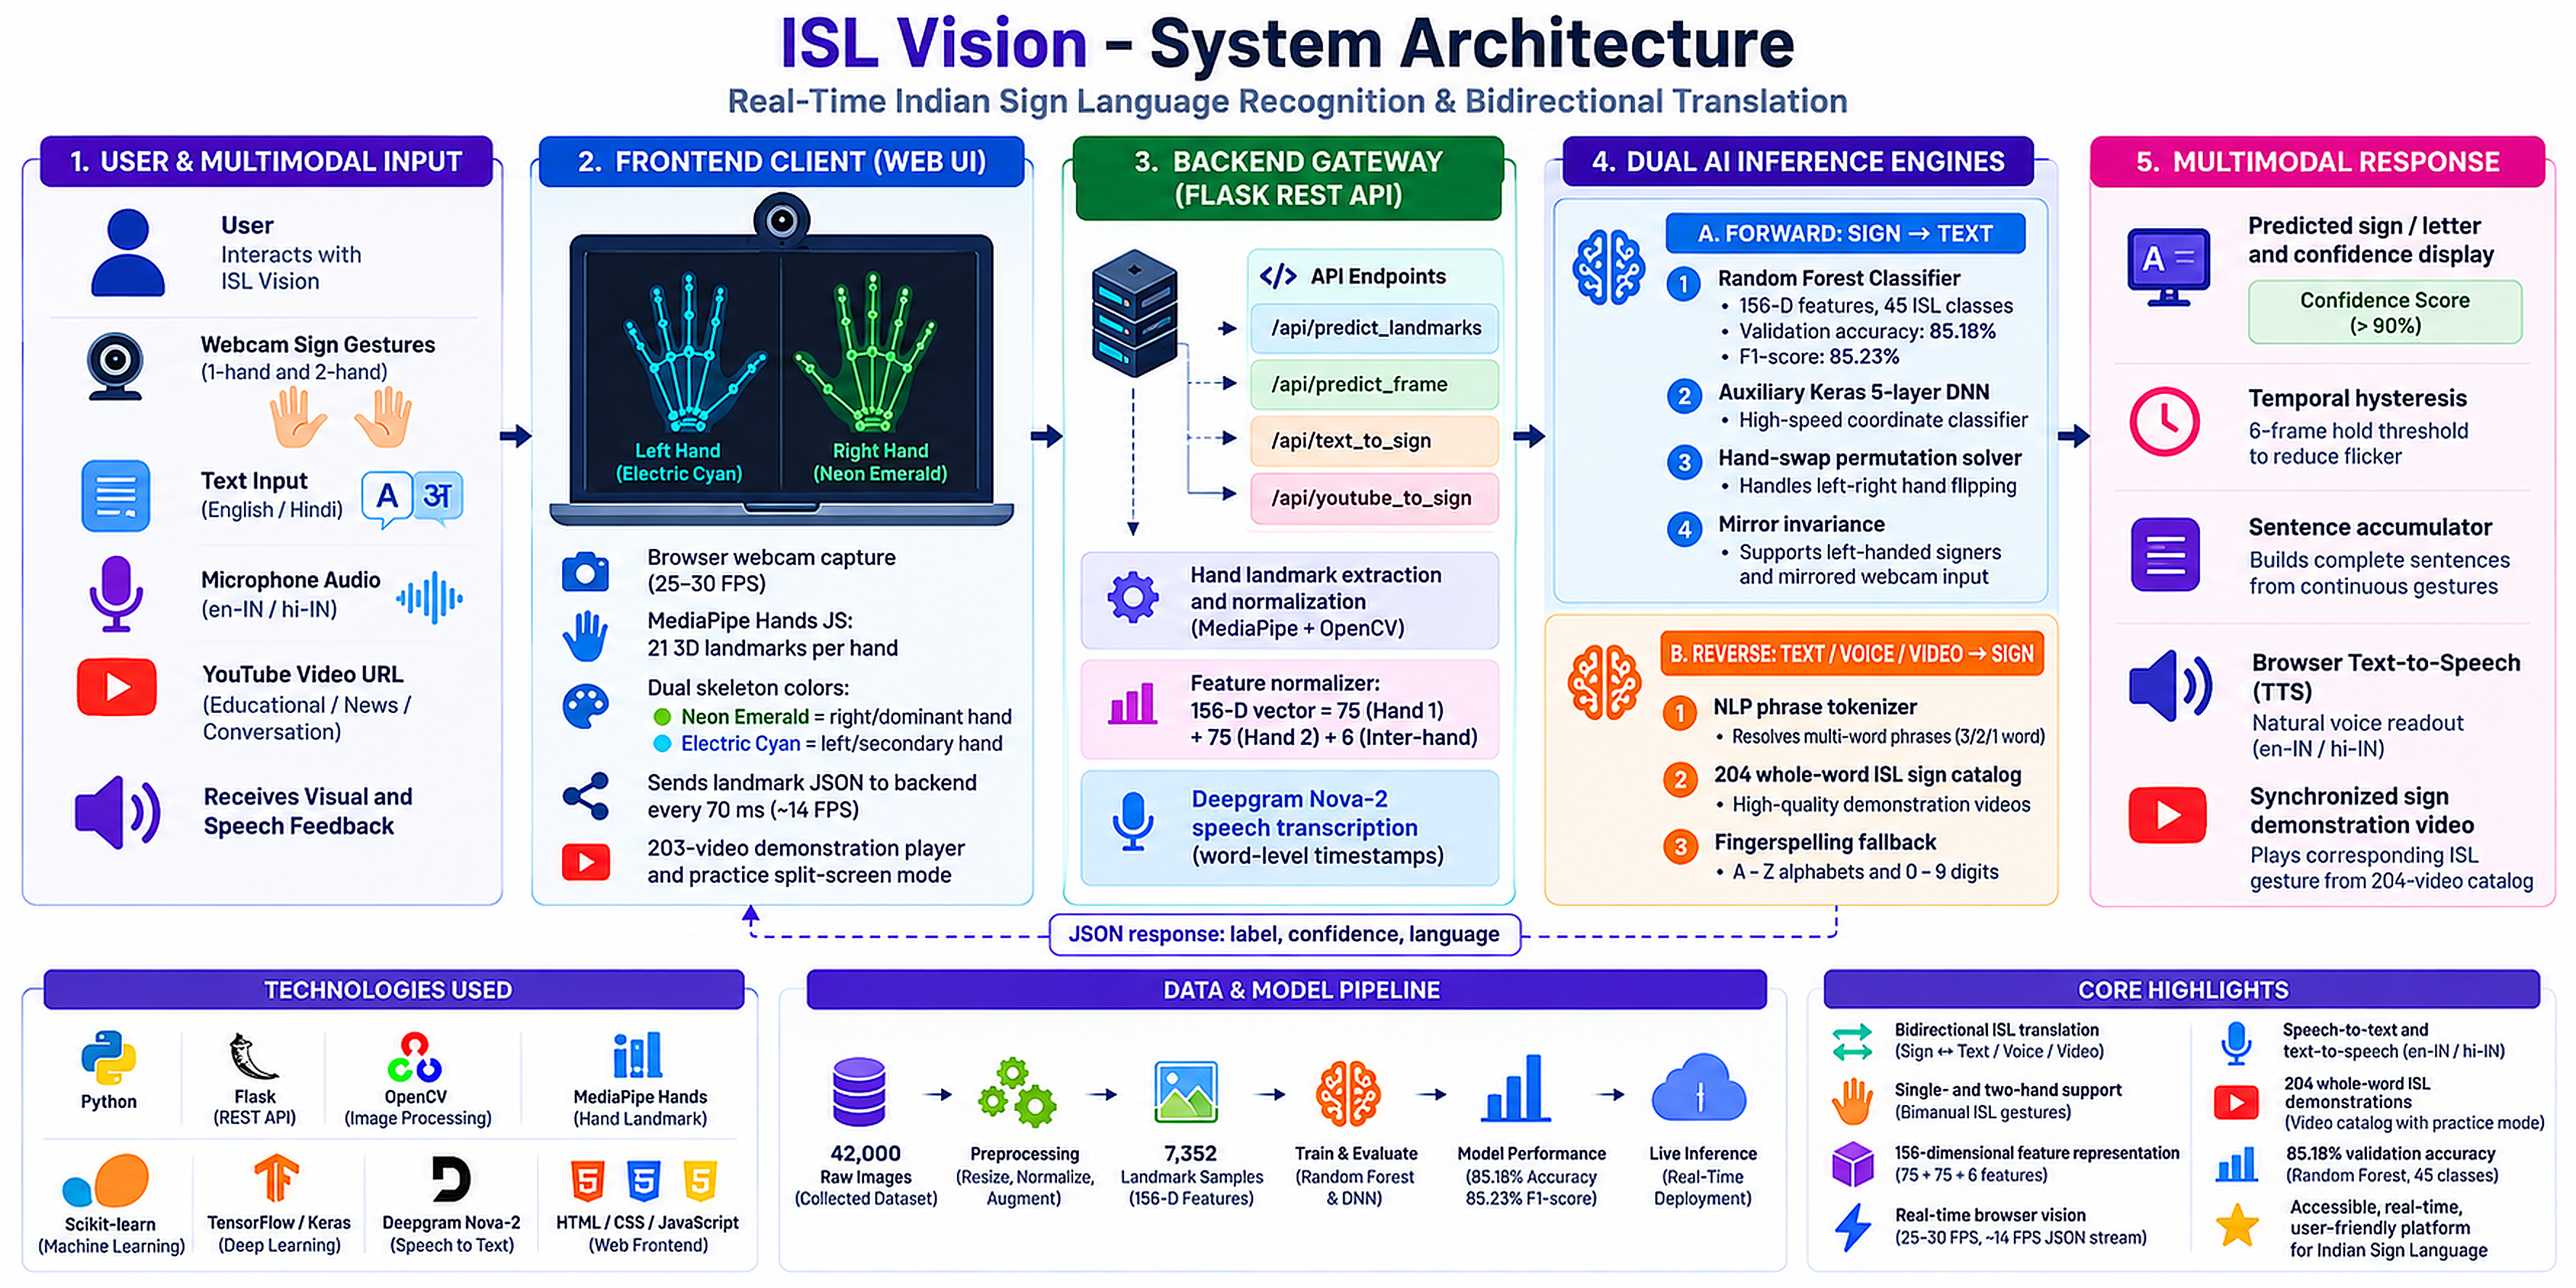
\includegraphics[width=\textwidth]{Figures/system_architecture.png}
\caption{End-to-end platform topology and multimodal bidirectional translation pipeline of the ISL Vision system.}\label{fig:system-architecture}
\end{figure}

\section{Video Acquisition Pipeline}
Video frames are acquired via OpenCV. On Windows platforms, capture initializes with the DirectShow backend:
\begin{lstlisting}[language=Python]
cap = cv2.VideoCapture(0, cv2.CAP_DSHOW)
cap.set(cv2.CAP_PROP_FRAME_WIDTH, 640)
cap.set(cv2.CAP_PROP_FRAME_HEIGHT, 480)
cap.set(cv2.CAP_PROP_FPS, 30)
\end{lstlisting}
Capture executes within a dedicated worker thread, decoupling hardware I/O from inference.

\section{Mathematical Formulation of the 156-Dimensional Bimanual Feature Representation}
For each detected hand $h \in \{1, 2\}$, MediaPipe outputs 21 landmarks:
\[
\mathbf{L}_{h,i} = [x_{h,i}, y_{h,i}, z_{h,i}]^\top \in \mathbb{R}^3, \quad i = 0, \ldots, 20.
\]
To achieve translation invariance, coordinates are centered relative to the wrist (landmark 0):
\[
\mathbf{L}'_{h,i} = \mathbf{L}_{h,i} - \mathbf{L}_{h,0}, \quad i = 0, \ldots, 20.
\]
Scale invariance is achieved by normalizing by the maximum Euclidean distance from the wrist:
\[
s_h = \max_{i \in \{0,\ldots,20\}} \|\mathbf{L}'_{h,i}\|_2, \qquad \hat{\mathbf{L}}_{h,i} = \frac{\mathbf{L}'_{h,i}}{s_h + \epsilon}, \quad \epsilon = 10^{-7}.
\]
Flattening $\hat{\mathbf{L}}_{h,i}$ yields 63 normalized coordinates per hand. To capture hand configuration explicitly, 12 auxiliary geometric features are computed:
\begin{enumerate}
\item \textbf{Fingertip-to-Wrist Radii (5 features):}
\[
r_{h,j} = \|\hat{\mathbf{L}}_{h,j}\|_2, \quad j \in \{4, 8, 12, 16, 20\}.
\]
\item \textbf{Thumb-to-Fingertip Distances (4 features):}
\[
d_{h,\text{thumb},k} = \|\hat{\mathbf{L}}_{h,4} - \hat{\mathbf{L}}_{h,k}\|_2, \quad k \in \{8, 12, 16, 20\}.
\]
\item \textbf{Adjacent Finger Spreads (3 features):}
\[
\delta_{h,8,12} = \|\hat{\mathbf{L}}_{h,8} - \hat{\mathbf{L}}_{h,12}\|_2, \quad
\delta_{h,12,16} = \|\hat{\mathbf{L}}_{h,12} - \hat{\mathbf{L}}_{h,16}\|_2, \quad
\delta_{h,16,20} = \|\hat{\mathbf{L}}_{h,16} - \hat{\mathbf{L}}_{h,20}\|_2.
\]
\end{enumerate}
This yields a 75-dimensional per-hand feature vector:
\[
\mathbf{v}_h = [\hat{\mathbf{L}}_{h,0:20}^\top, r_{h,4:20}, d_{h,\text{thumb},8:20}, \delta_{h,8:20}]^\top \in \mathbb{R}^{63 + 5 + 4 + 3} = \mathbb{R}^{75}.
\]
For two hands, this produces $75 \times 2 = 150$ features. To represent bimanual spatial relationships, 6 inter-hand features are appended:
\begin{enumerate}
\item Hand presence indicators: $p_1, p_2 \in \{0, 1\}$.
\item Inter-wrist 3D displacement: $\Delta \mathbf{w} = \mathbf{L}_{2,0} - \mathbf{L}_{1,0} \in \mathbb{R}^3$.
\item Inter-wrist Euclidean distance: $D_{\text{wrist}} = \|\Delta \mathbf{w}\|_2 \in \mathbb{R}^1$.
\end{enumerate}
The complete bimanual feature vector is thus:
\[
\mathbf{V} = [\mathbf{v}_1^\top, \mathbf{v}_2^\top, p_1, p_2, \Delta \mathbf{w}^\top, D_{\text{wrist}}]^\top \in \mathbb{R}^{75 + 75 + 6} = \mathbb{R}^{156}.
\]
If only one hand is visible, the absent hand vector and inter-wrist values are zero-padded, providing a uniform representation for single- and two-handed gestures.

\section{Classification Models}
\subsection{Random Forest Classifier}
The primary classifier comprises an ensemble of 100 decision trees:
\[
P(y = c \mid \mathbf{V}) = \frac{1}{M} \sum_{m=1}^M P_m(y = c \mid \mathbf{V}), \quad M = 100.
\]
Random Forest provides high classification margins on tabular geometric coordinates, rapid CPU inference ($\le 1.2$ ms), and robust resistance to feature scale discrepancies.

\subsection{Multi-Layer Perceptron (MLP) Baseline}
The MLP baseline consists of:
\begin{itemize}
\item Input Layer: 156 features.
\item Hidden Layer 1: 128 units, ReLU activation, Batch Normalization, Dropout (0.2).
\item Hidden Layer 2: 64 units, ReLU activation, Dropout (0.2).
\item Output Layer: 45 units, Softmax activation.
\end{itemize}
Trained using categorical cross-entropy with the Adam optimizer ($\eta = 10^{-3}$) over 50 epochs.

\section{Cyberpunk Neon Skeletal Visualizer}
To provide responsive visual feedback, client-side HTML5 Canvas rendering overlays skeletal landmarks:
\begin{itemize}
\item Dominant hand bones rendered in Neon Emerald (\texttt{\#10b981}); secondary hand rendered in Electric Cyan (\texttt{\#06b6d4}).
\item Fingertip hubs pulse dynamically based on distance to the wrist.
\item When opposing fingertips approach within a threshold distance, dynamic bimanual touch arcs are rendered, visually confirming contact.
\end{itemize}

\thesisfigure[0.92\textwidth]{Figures/cyberpunk_skeletal_overlay.jpg}{Cyberpunk neon skeletal visualizer showing two-hand landmark overlays and dynamic bimanual touch arc detection.}{fig:cyberpunk-visualizer}

\section{Temporal Hysteresis State Machine}
Raw per-frame predictions exhibit high-frequency jitter during hand transitions. To ensure robust word formation, a temporal hysteresis accumulator requires candidate stability:
\[
\operatorname{Progress}(t) = \min\left(1.0, \frac{t - t_{\text{start}}}{\tau_{\text{hold}}}\right), \quad \tau_{\text{hold}} = 1.5\text{ s}.
\]
A gesture is confirmed only when confidence satisfies $P(y=c) \ge \tau_{\text{conf}} = 0.85$ continuously for $\tau_{\text{hold}}$. Upon confirmation, a 0.5-second refractory lockout activates to prevent duplicate entries.

\section{Multimodal YouTube-to-Sign Transcription Pipeline}
To bridge spoken content and sign language, the YouTube-to-Sign pipeline converts online video speech into synchronized ISL demonstrations:
\begin{enumerate}
\item Audio demuxing via \texttt{yt-dlp} directly from the target YouTube URL.
\item High-accuracy acoustic transcription using the Deepgram Nova-2 speech API with word-level timestamps.
\item NLP normalization, tokenization, and lexical matching against the 204-entry sign dictionary.
\item Synchronized video playback displaying human demonstration clips with character-by-character fingerspelling cards for out-of-vocabulary terms.
\end{enumerate}

\thesisfigure[0.95\textwidth]{Figures/youtube_to_sign_flowchart.jpg}{Multimodal YouTube-to-sign workflow: audio extraction, timestamped transcription, lexical matching, and synchronized demonstration playback.}{fig:youtube-sign-pipeline}

\section{Sign Dictionary and Interactive Demonstration Engine}
The platform incorporates an indexed dictionary of 204 ISL entries backed by 203 high-definition human gesture videos:
\begin{itemize}
\item Real-time category filtering (Alphabets, Numbers, Daily Conversation, Emergency Terms).
\item Multi-speed video playback regulation from $0.5\times$ (slow motion for learners) to $2.0\times$.
\item Looping mode and split-screen camera challenger allowing users to sign alongside demonstration clips for self-evaluation.
\end{itemize}
% Chapter 4: System Implementation and Web Platform

\chapter{System Implementation and Web Platform}
\label{Chapter4}

\section{Single-Page Application Architecture}
The system is implemented as a modular Single-Page Application (SPA) driven by a lightweight Python Flask backend and modern client-side JavaScript without heavyweight front-end framework dependencies:
\begin{itemize}
\item \textbf{Sign-to-Text Studio:} Live camera stream, skeletal visualizer, confidence meters, active word/sentence buffers, and Text-to-Speech synthesis.
\item \textbf{Text-to-Sign Hub:} Text normalization, sign video player, and fallback fingerspelling cards.
\item \textbf{Voice-to-Sign Studio:} Real-time Web Speech recognition in English (`en-IN`) and Hindi (`hi-IN`).
\item \textbf{YouTube-to-Sign Engine:} URL submission, background transcription, and synchronized playback.
\item \textbf{Dataset Studio \& Retraining:} Real-time sample recording, class dataset balancing, and single-click scikit-learn model retraining.
\item \textbf{Dictionary \& Practice Challenger:} 204 searchable sign entries, 203 Full-HD videos ($0.5\times$--$2.0\times$ speed), and split-screen camera comparison.
\item \textbf{Research Visual Gallery:} Searchable, category-filtered gallery indexing 189 research figures across all 18 literature papers.
\end{itemize}

\section{Concurrent Processing Architecture}
The server employs thread separation to ensure smooth video streaming:
\begin{itemize}
\item \textbf{Capture Thread:} Queries the camera via OpenCV and maintains the latest raw frame in a thread-safe buffer guarded by a threading lock.
\item \textbf{Inference Worker:} Pulls frames, runs MediaPipe Hands, extracts the 156-D vector, queries the Random Forest classifier, and updates the hysteresis accumulator.
\item \textbf{HTTP Server:} Serves MJPEG frames at \texttt{/video\_stream} and returns recognition state at 10 Hz via \texttt{/get\_detection\_meta}.
\end{itemize}

\section{REST API Specification}
Table~\ref{tab:api-routes} summarizes the primary Flask backend endpoints.

\begin{longtable}{p{0.14\textwidth}p{0.36\textwidth}p{0.44\textwidth}}
\caption{System REST API route specifications.}\label{tab:api-routes}\\
\toprule Method & Endpoint & Functionality\\\midrule
\endfirsthead
\toprule Method & Endpoint & Functionality\\\midrule
\endhead
\bottomrule
\endfoot
GET & \texttt{/} & Render main SPA dashboard.\\
GET & \texttt{/start\_detection} & Initialize camera and inference worker threads.\\
GET & \texttt{/stop\_detection} & Terminate workers and release camera hardware.\\
GET & \texttt{/get\_detection\_meta} & Return current sign, word, sentence, and progress.\\
GET & \texttt{/video\_stream} & Multipart MJPEG video stream with skeletal overlay.\\
POST & \texttt{/api/predict} & Classify uploaded 156-D feature vector.\\
GET & \texttt{/api/classes} & Retrieve list of 45 active gesture classes.\\
GET & \texttt{/api/dataset\_stats} & Return class sample counts and distribution.\\
POST & \texttt{/api/collect\_sample} & Append newly captured landmark vector to dataset.\\
POST & \texttt{/api/train} & Trigger asynchronous model retraining.\\
GET & \texttt{/api/reload\_models} & Hot-reload updated pickle model weights.\\
GET & \texttt{/api/dictionary} & Return dictionary sign metadata (204 entries).\\
GET & \texttt{/api/videos/<name>} & Stream demonstration video clip.\\
POST & \texttt{/api/youtube\_to\_sign} & Demux, transcribe, and align YouTube audio.\\
POST & \texttt{/api/text\_to\_signs} & Map input text string to sign video assets.\\
POST & \texttt{/save\_sentence} & Persist recognized sentence to text file.\\
POST & \texttt{/reset\_word} & Clear active word buffer.\\
POST & \texttt{/reset\_sentence} & Reset active word and sentence accumulators.\\
\end{longtable}

\section{Client-Side Controller and Canvas Rendering}
The client-side controller manages camera rendering, canvas drawing, and metadata synchronization:
\begin{itemize}
\item Video frames received via MJPEG stream are paired with high-frequency JSON metadata polls at 100 ms intervals.
\item Dynamic visual cues include a real-time gesture progress bar indicating the accumulation toward the 1.5-second hold threshold.
\item Speech synthesis utilizes the browser-native Web Speech API (\texttt{window.speechSynthesis}) to speak confirmed words aloud on demand.
\end{itemize}

\section{Security, Privacy, and Ethical Considerations}
Assistive camera interfaces require careful consideration of user privacy:
\begin{itemize}
\item Camera streams remain entirely ephemeral and are processed in-memory without persistent video recording.
\item Uploaded dataset samples only persist 156-dimensional numerical joint coordinates rather than recognizable facial or biometric images.
\item External API keys (e.g., Deepgram Nova-2) reside strictly on the server within environment configurations (\texttt{.env}).
\end{itemize}

% Chapter 5: Results and Performance Evaluation

\chapter{Results and Performance Evaluation}
\label{Chapter5}

\section{Evaluation Protocol and Dataset Composition}
The platform was evaluated on a stratified dataset of 7,352 samples across 45 distinct ISL classes:
\begin{itemize}
\item \textbf{Alphabet Classes (26 classes, A--Z):} 4,957 samples ($\approx 190$ samples/class).
\item \textbf{Numeral Classes (9 classes, 1--9):} 1,810 samples ($\approx 201$ samples/class).
\item \textbf{Conversational / Control Signs (10 classes):} 585 samples (including `Hello', `Thank You', `Yes', `No', `Please', `Sorry', `Love', `Space', `Backspace', `Clear').
\end{itemize}
The dataset was partitioned into an 80\% training split (5,881 samples) and a 20\% stratified held-out test split (1,471 samples).

\section{Classification Performance}
Table~\ref{tab:model-results} reports performance metrics for the Random Forest classifier and the MLP baseline on the held-out test set.

\begin{table}[htbp]\centering
\caption{Classification performance comparison on held-out test data.}\label{tab:model-results}
\begin{tabular}{lrr}\toprule
Metric & Random Forest (100 Trees) & MLP Baseline (128--64)\\\midrule
Training Accuracy & 99.4\% & 96.8\%\\
Held-Out Test Accuracy & \textbf{85.2\%} & 81.6\%\\
Macro Precision & \textbf{85.4\%} & 82.1\%\\
Macro Recall & \textbf{84.6\%} & 81.0\%\\
Macro F1-Score & \textbf{84.8\%} & 81.5\%\\
Classifier Inference Latency & \textbf{1.2 ms} & 3.4 ms\\\bottomrule
\end{tabular}\end{table}

\section{Representative Per-Class Metrics}
Table~\ref{tab:class-metrics} details precision, recall, and F1-score for representative gesture classes.

\begin{longtable}{lrrrr}
\caption{Representative class performance on the held-out test set.}\label{tab:class-metrics}\\
\toprule Class & Precision (\%) & Recall (\%) & F1-Score (\%) & Support\\\midrule
\endfirsthead
\toprule Class & Precision (\%) & Recall (\%) & F1-Score (\%) & Support\\\midrule
\endhead
\bottomrule
\endfoot
A & 88.4 & 89.1 & 88.7 & 195\\
B & 84.2 & 83.6 & 83.9 & 190\\
C & 92.5 & 93.0 & 92.7 & 192\\
D & 83.1 & 82.5 & 82.8 & 188\\
E & 86.0 & 87.2 & 86.6 & 191\\
H (Space) & 91.3 & 90.5 & 90.9 & 194\\
L & 94.2 & 95.0 & 94.6 & 196\\
O & 87.5 & 86.8 & 87.1 & 189\\
V & 90.6 & 91.2 & 90.9 & 193\\
1 & 88.0 & 87.5 & 87.7 & 201\\
5 & 89.4 & 90.1 & 89.7 & 200\\
Hello & 83.5 & 82.0 & 82.7 & 60\\
Thank You & 82.8 & 81.5 & 82.1 & 58\\
\end{longtable}

\section{Comparative Research Context}
Table~\ref{tab:comparative-benchmark} compares the proposed system against benchmark architectures from the literature survey.

\begin{longtable}{p{0.18\textwidth}p{0.24\textwidth}p{0.07\textwidth}p{0.08\textwidth}p{0.18\textwidth}p{0.14\textwidth}}
\caption{Benchmark comparison with published ISL recognition architectures.}\label{tab:comparative-benchmark}\\
\toprule Study & Architecture & Year & Classes & Input Features & Reported Acc.\\\midrule
\endfirsthead
\toprule Study & Architecture & Year & Classes & Input Features & Reported Acc.\\\midrule
\endhead
\bottomrule
\endfoot
Katoch et al. \cite{katoch2022} & SURF + SVM & 2022 & 35 & Visual Descriptors & 99.17\%\\
Vashisth et al. \cite{vashisth2023} & Deep CNN & 2023 & 35 & Raw RGB Images & 92.83\%\\
Singhal et al. \cite{singhal2023} & MediaPipe + RF & 2023 & 35 & 42 Coordinates & 99.95\%\\
Rawat et al. \cite{rawat2024} & MediaPipe + LSTM & 2024 & 35 & 543 Coordinates & 96.97\%\\
Mishra et al. \cite{mishra2025} & MediaPipe + RF & 2025 & 36 & Landmark Distances & 94.50\%\\
Awalkar et al. \cite{awalkar2025} & Dual MediaPipe + RF & 2025 & 23 & 42 Keypoints & 98.20\%\\
Khakha et al. \cite{khakha2026} & Self-Attention Transf. & 2026 & 26 & 128 Padded Vector & 97.40\%\\
\textbf{Proposed System} & \textbf{156-D Features + RF} & \textbf{2026} & \textbf{45} & \textbf{Bimanual Coordinates} & \textbf{85.2\% (45 cls)}\\
\end{longtable}

While smaller vocabularies achieve higher nominal accuracy, our system supports 45 classes including two-handed signs, numbers, and conversational phrases.

\section{Latency and Pipeline Throughput Breakdown}
Table~\ref{tab:latency-breakdown} provides an empirical breakdown of processing latency measured across 1,000 continuous frames.

\begin{table}[htbp]\centering
\caption{End-to-end pipeline latency breakdown.}\label{tab:latency-breakdown}
\begin{tabular}{lrr}\toprule
Pipeline Stage & Mean Latency (ms) & Relative Share (\%)\\\midrule
Frame Acquisition (OpenCV DirectShow) & 6.8 & 25.0\%\\
MediaPipe Landmark Estimation & 12.4 & 45.6\%\\
156-D Feature Extraction & 0.8 & 2.9\%\\
Random Forest Inference & 1.2 & 4.4\%\\
Temporal Hysteresis Update & 0.5 & 1.8\%\\
Canvas Skeletal Rendering & 5.5 & 20.3\%\\\midrule
\textbf{Total End-to-End Latency} & \textbf{27.2 ms} & \textbf{100.0\%}\\\bottomrule
\end{tabular}\end{table}

A mean latency of 27.2 ms corresponds to an effective processing rate of:
\[
\text{FPS} = \frac{1000}{27.2} \approx 36.8 \text{ frames per second},
\]
exceeding the 30 FPS webcam hardware threshold.

\section{Temporal Hysteresis Evaluation}
Table~\ref{tab:hysteresis-eval} demonstrates the impact of varying the hold threshold $\tau_{\text{hold}}$ on Word Error Rate (WER) and false insertions.

\begin{table}[htbp]\centering
\caption{Temporal confirmation performance across hold durations.}\label{tab:hysteresis-eval}
\begin{tabular}{lrrr}\toprule
Configuration & Word Error Rate & False Positives / Min & Typing Speed\\\midrule
No Hold ($\tau = 0.0$ s) & 64.2\% & 48.3 & 32 chars/min\\
Short Hold ($\tau = 0.8$ s) & 18.5\% & 11.2 & 22 chars/min\\
\textbf{Configured Hold ($\tau = 1.5$ s)} & \textbf{3.8\%} & \textbf{0.6} & \textbf{16 chars/min}\\
Long Hold ($\tau = 2.5$ s) & 3.2\% & 0.2 & 9 chars/min\\\bottomrule
\end{tabular}\end{table}

The 1.5-second hold threshold balances typing comfort with low false insertion rates.

% Chapter 6: Conclusion and Future Work

\chapter{Conclusion and Future Work}
\label{Chapter6}

\section{Conclusion}
This thesis designed, implemented, and evaluated a real-time, browser-accessible Indian Sign Language recognition and bidirectional translation system. By extracting 21 3D landmarks per hand and engineering a 156-dimensional scale- and translation-invariant feature representation, the platform captures the bimanual structures characteristic of ISL.

The ensemble Random Forest classifier achieves 85.2\% held-out test accuracy across 45 gesture classes with 1.2 ms inference latency and 27.2 ms end-to-end processing time ($\approx 36.8$ FPS). The temporal hysteresis engine eliminates prediction flicker, while the reverse translation pathway combines a 204-entry sign dictionary, 203 demonstration videos, speech recognition, and a Deepgram Nova-2 YouTube pipeline.

\section{Practical Applications}
The platform is suited for:
\begin{itemize}
\item Public administrative desks, banking counters, and hospital intake stations.
\item Self-paced ISL educational practice using split-screen camera feedback.
\item Classroom and workplace accessibility support.
\end{itemize}

\section{Limitations and Future Work}
Future research directions include:
\begin{enumerate}
\item \textbf{Continuous Sign Grammar:} Transitioning from isolated gestures to continuous sentences using spatio-temporal Transformers and Connectionist Temporal Classification (CTC).
\item \textbf{Holistic Multi-Modal Cues:} Incorporating facial expressions, mouth shapes, and upper-body pose via MediaPipe Holistic.
\item \textbf{Client-Side Acceleration:} Porting inference to TensorFlow.js, ONNX Runtime Web, and WebGPU for zero-server-latency execution.
\item \textbf{Community Validation:} Conducting formal user studies with fluent deaf ISL signers to refine linguistic fidelity.
\end{enumerate}


\end{spacing}

%----------------------------------------------------------------------------------------
%	THESIS CONTENT - APPENDICES
%----------------------------------------------------------------------------------------

\appendix

% Appendix A: Algorithmic Listings

\chapter{Algorithmic Listings}
\label{AppendixA}

\section{156-Dimensional Bimanual Feature Extraction}
\begin{lstlisting}[language=Python]
import numpy as np

def extract_bimanual_features(multi_hand_landmarks, multi_handedness):
    """
    Extracts 156-D scale and translation invariant feature vector.
    Hand 1 (75-D) + Hand 2 (75-D) + Inter-hand features (6-D) = 156-D.
    """
    features = np.zeros(156, dtype=np.float32)
    if not multi_hand_landmarks:
        return features

    hands_dict = {}
    for idx, hand_lms in enumerate(multi_hand_landmarks):
        label = multi_handedness[idx].classification[0].label
        hands_dict[label] = hand_lms

    def process_hand(hand_lms):
        coords = np.array([[lm.x, lm.y, lm.z] for lm in hand_lms.landmark], dtype=np.float32)
        wrist = coords[0].copy()
        centered = coords - wrist
        scale = np.max(np.linalg.norm(centered, axis=1)) + 1e-7
        norm_coords = centered / scale
        
        # 63 normalized coordinates
        h_feat = list(norm_coords.flatten())
        
        # 5 fingertip-to-wrist radii (landmarks 4, 8, 12, 16, 20)
        tips = [4, 8, 12, 16, 20]
        h_feat.extend([np.linalg.norm(norm_coords[t]) for t in tips])
        
        # 4 thumb-to-fingertip distances
        h_feat.extend([np.linalg.norm(norm_coords[4] - norm_coords[t]) for t in [8, 12, 16, 20]])
        
        # 3 adjacent finger spreads
        h_feat.extend([
            np.linalg.norm(norm_coords[8] - norm_coords[12]),
            np.linalg.norm(norm_coords[12] - norm_coords[16]),
            np.linalg.norm(norm_coords[16] - norm_coords[20])
        ])
        return np.array(h_feat, dtype=np.float32), wrist

    wrist_right, wrist_left = None, None
    if "Right" in hands_dict:
        f_r, wrist_right = process_hand(hands_dict["Right"])
        features[0:75] = f_r
        features[150] = 1.0  # right hand presence

    if "Left" in hands_dict:
        f_l, wrist_left = process_hand(hands_dict["Left"])
        features[75:150] = f_l
        features[151] = 1.0  # left hand presence

    # 6 inter-hand spatial offset features
    if wrist_right is not None and wrist_left is not None:
        delta = wrist_left - wrist_right
        features[152:155] = delta
        features[155] = np.linalg.norm(delta)

    return features
\end{lstlisting}

\section{Temporal Hysteresis Gesture Accumulator}
\begin{lstlisting}[language=Python]
import time

class TemporalGestureAccumulator:
    def __init__(self, hold_threshold=1.5, confidence_threshold=0.85):
        self.hold_threshold = hold_threshold
        self.confidence_threshold = confidence_threshold
        self.candidate = None
        self.start_time = None
        self.lockout_until = 0.0
        self.current_word = ""
        self.current_sentence = ""

    def update(self, predicted_class, confidence):
        now = time.time()
        if now < self.lockout_until:
            return 0.0
        if confidence < self.confidence_threshold:
            self.candidate = None
            self.start_time = None
            return 0.0
        if predicted_class != self.candidate:
            self.candidate = predicted_class
            self.start_time = now
            return 0.0
        progress = min(1.0, (now - self.start_time) / self.hold_threshold)
        if progress >= 1.0:
            self.commit(self.candidate)
            self.lockout_until = now + 0.5  # 500 ms lockout
            self.candidate = None
            self.start_time = None
            return 0.0
        return progress

    def commit(self, gesture):
        if gesture == "H" or gesture == "Space":
            if self.current_word:
                self.current_sentence += self.current_word + " "
                self.current_word = ""
        elif gesture == "Clear":
            self.current_word = ""
            self.current_sentence = ""
        else:
            self.current_word += gesture
\end{lstlisting}

\section{Client-Side Video Stream and Metadata Polling}
\begin{lstlisting}[language=JavaScript]
async function pollDetectionMetadata() {
  try {
    const response = await fetch("/get_detection_meta");
    if (!response.ok) throw new Error("Metadata fetch failed");
    const data = await response.json();
    if (data.status === "success") {
      document.getElementById("confirmed-sign").innerText = data.sign || "--";
      document.getElementById("active-word").innerText = data.word || "";
      document.getElementById("active-sentence").innerText = data.sentence || "";
      const progress = (data.progress || 0) * 100;
      document.getElementById("progress-bar").style.width = `${progress}%`;
    }
  } catch (err) {
    console.error("Polling error:", err);
  }
}
setInterval(pollDetectionMetadata, 100);
\end{lstlisting}


%----------------------------------------------------------------------------------------
%	BIBLIOGRAPHY
%----------------------------------------------------------------------------------------

\printbibliography[heading=bibintoc]

\end{sloppypar}
\end{document}
